\documentclass[t, aspectratio=169]{beamer}
\usepackage{amsmath,amsfonts,amsthm,amstext,amssymb, xcolor, tikz, pgf, mathrsfs, polynom, pifont, tabto}

% ----------------------------------------------------------
% Theme Setup

% Use Metropolis Theme
\usetheme[numbering=fraction]{metropolis}
\setbeamertemplate{blocks}[rounded][shadow=false]
\makeatletter
\setlength{\metropolis@titleseparator@linewidth}{1pt}
\makeatother

% Define Colors
\definecolor{chargerblue}{HTML}{002764}
\definecolor{chargerred}{HTML}{e02034}
\definecolor{bggray}{HTML}{d0d3d4}

% Set Colors
\setbeamercolor{title}{fg=chargerblue}
\setbeamercolor{background canvas}{bg=white}
\setbeamercolor{title separator}{fg=chargerred}
\setbeamercolor{structure}{fg=chargerblue}
\setbeamercolor{frametitle}{fg=white, bg=chargerblue}
\setbeamercolor*{normal text}{fg=chargerblue}
\setbeamercolor*{block body}{bg=bggray}
\setbeamercolor*{block title}{bg=chargerblue, fg=white}
% ----------------------------------------------------------

% ----------------------------------------------------------
% Custom Definitions, Commands, Environments, etc.

% Sets of numbers
\def\R{\mathbb{R}} % The reals
\def\N{\mathbb{N}} % The naturals
\def\Z{\mathbb{Z}} % The integers
\def\Q{\mathbb{Q}} % The rationals

% Blank space
\newcommand{\blank}[1]{\underline{\hspace{#1}}} % Blank space

% Change font colors
\newcommand{\cyan}[1]{{\color{cyan}{#1}}} % Changes font to cyan
\newcommand{\red}[1]{{\color{red}{#1}}} % Changes font to red
\newcommand{\magenta}[1]{{\color{magenta}{#1}}} % Changes font to magenta
\newcommand{\orange}[1]{{\color{orange}{#1}}} % Changes font to orange
\newcommand{\yellow}[1]{{\color{yellow}{#1}}} % Changes font to yellow
\newcommand{\violet}[1]{{\color{violet}{#1}}} % Changes font to violet
\newcommand{\green}[1]{{\color{green}{#1}}} % Changes font to green
\newcommand{\blue}[1]{{\color{blue}{#1}}} % Changes font to blue
\newcommand{\white}[1]{{\color{white}{#1}}} % Changes font to white

% Fitted inclusion symbols
\newcommand{\fp}[1]{\left({#1}\right)} % Fitted parentheses around content
\newcommand{\fb}[1]{\left[{#1}\right]} % Fitted brackets
\newcommand{\lhoi}[1]{\left({#1}\right]} % Left half-open interval
\newcommand{\rhoi}[1]{\left[{#1}\right)} % Right half-open interval
\newcommand{\set}[1]{\left\{{#1}\right\}} % Fitted braces (useful for sets)
\newcommand{\av}[1]{\left|{#1}\right|} % Fitted absolute value bars

% Augmented Matrix Environment
\newenvironment{amatrix}[1]{%
	\left[\begin{array}{@{}*{#1}{c}|c@{}}
	}{%
	\end{array}\right]
}

% Miscellaneous
\def\then{\Rightarrow}
\def\to{\rightarrow}
\def\d{^{\circ}}
\newcommand{\?}{\stackrel{?}{=}}
\newcommand{\cmark}{\text{ \ding{51}}}
\newcommand{\xmark}{\text{ \ding{55}}}

% Coordinate Plane (Four-Quadrant)
\def\coordplane {
	\begin{tikzpicture}        \draw[step=0.25cm,black,very thin,opacity=0.25] (-2.5cm, -2.5cm) grid (2.5cm, 2.5cm);
		\draw[<->,thick,black] (-2.5cm, 0) -- (2.5cm, 0) node[anchor=north west,pos=0.94,font=\scriptsize]{$x$};
		\draw[<->,thick,black] (0,-2.5cm) -- (0, 2.5cm) node[anchor=south east,font=\scriptsize,pos=0.94]{$y$};
	\end{tikzpicture}
}

% Coordinate Plane (One-Quadrant)
\def\onequad {
	\begin{tikzpicture}
		\draw[step=0.25cm, black, very thin, opacity=0.25] (0,0) grid (7.5cm,5cm);
		\draw[->, thick, black] (0,0) -- (7.5cm, 0) node[anchor=north west,font=\scriptsize,pos=0.94]{$x$};
		\draw[->, black, thick] (0,0) -- (0,5cm) node[anchor=south east,font=\scriptsize,pos=0.94]{$y$};
	\end{tikzpicture}
}
% ----------------------------------------------------------

% ----------------------------------------------------------
% Presentation Information
\title[4-2]{Addition Rules for Probability}
\subtitle{Section 4-2}
\author{Jacob Ayers}
\institute{Lesson \#10}
\date{MAT 110}
% ----------------------------------------------------------

\begin{document}
	
	% Slide 1 (Title Slide)
	\begin{frame}
		\titlepage
	\end{frame}
	
	% Slide 2 (Objectives)
	\begin{frame}{Objectives}
		\begin{itemize}
			\item Use the addition rules of probability to find the probabilities of ``or" statements
		\end{itemize}
	\end{frame}

	\begin{frame}{The Word ``Or"}
		Often, we want to know the probability that multiple events will occur. \pause
		
		In this lesson, we will focus on finding the probability of an ``or" statement. \pause
		
		In mathematics, we use the ``inclusive" definition of ``or.". \pause
		
		This means that ``A or B" is true in each of the following cases: \begin{enumerate}[1)]
			\item A is true
			\item B is true
			\item A and B are both true
		\end{enumerate}
	\end{frame}

	\begin{frame}{Mutually Exclusive Events}
		Two events are \textit{mutually exclusive} if they cannot occur at the same time. \pause
		
		Example: Rolling a 4 and rolling a 6 are mutually exclusive \pause \\
		Example: Drawing a spade and drawing a 6 are not mutually exclusive (could draw 6 of spades)
		
		Determine whether the two events are mutually exclusive. \begin{enumerate}[a)]
			\item Randomly selecting female student; randomly selecting student who is a junior \pause NO \pause
			\item Person has type A blood; Person has type O blood \pause YES \pause
			\item Rolling an odd number; Rolling a number less than 3 \pause NO \pause
			\item Select person under age 21; Select person over age 30 \pause YES
		\end{enumerate}
	\end{frame}

	\begin{frame}{Addition Rules of Probability}
		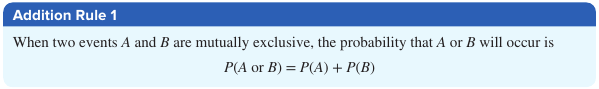
\includegraphics[width=5in]{add-1.png} \pause
		
		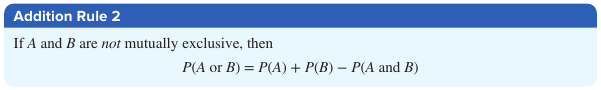
\includegraphics[width=5in]{add-2.png} \pause
		
		Note: I only recommend memorizing rule 2, since it also works when $A$ and $B$ are mutually exclusive ($P(A \text{ and } B) = 0$ in this case)
	\end{frame}

	\begin{frame}{Addition Rules of Probability}
		In the United States there are 59 different species of mammals that are endangered, 75 different species of birds that are endangered, and 68 species of fish that are endangered. If one animal is selected at random, find the probability that it is a mammal or a bird. \pause
		
		Note that these events are mutually exclusive (an animal cannot be both a mammal and a bird). \pause \begin{flalign*}
			P(\text{mammal or bird}) &= P(\text{mammal}) + P(\text{bird}) & \\
			&= \dfrac{59}{202} + \dfrac{75}{202} & \\
			&= \dfrac{134}{202} = \dfrac{67}{101}  & \\
			&\approx 0.663 \text{ or } 66.3\%
		\end{flalign*}
	\end{frame}

	\begin{frame}{Addition Rules of Probability}
		In a hospital unit, there are 8 nurses and 5 physicians; 7 nurses and 3 physicians are females. If a staff person is selected at random, find the probability that the subject is a physician or a female. \pause
		
		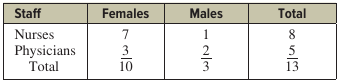
\includegraphics[width=3in]{hospital.png} \pause \begin{flalign*}
			P(\text{physician or female}) &= P(\text{physician}) + P(\text{female}) - P(\text{female physician}) & \\
			&= \dfrac{5}{13} + \dfrac{10}{13} - \dfrac{3}{13} & \\
			&= \dfrac{12}{13} \approx 0.923 \text{ or } 92.3\%
		\end{flalign*}
	\end{frame}

	\begin{frame}{Addition Rules of Probability}
		The table below represents the college degrees awarded in a recent academic year by gender.
		
		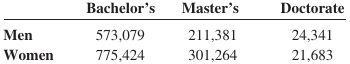
\includegraphics[width=2.5in]{grad-data.png}
		
		Choose a degree at random. Find the probability that it is a doctorate or a degree awarded to a man. \begin{flalign*}
			\onslide<2->{P(\text{doctorate or male}) &= P(\text{doctorate}) + P(\text{male}) - P(\text{male doctorate}) & \\}
			\onslide<3->{&= \dfrac{46024}{1907172} + \dfrac{808801}{1907172} - \dfrac{24341}{1907172} & \\}
			\onslide<4->{&= \dfrac{830484}{1907172} & \\}
			\onslide<5->{&\approx 0.435}
		\end{flalign*}
	\end{frame}

	\begin{frame}{Addition Rules of Probability}
		The number of multiple births in the United States for a recent year indicated that there were 128,665 sets of twins, 7110 sets of triplets, 468 sets of quadruplets, and 85 sets of quintuplets. Choose one set of siblings at random. \begin{enumerate}[a)]
			\item Find the probability that it represented more than two babies.
			\item Find the probability that it represented quads or quints.
			\item Choose one baby from these multiple births. What is the probability that the baby was a triplet?
		\end{enumerate}
	\end{frame}

	\begin{frame}{Addition Rules of Probability}
		The number of multiple births in the United States for a recent year indicated that there were 128,665 sets of twins, 7110 sets of triplets, 468 sets of quadruplets, and 85 sets of quintuplets. Choose one set of siblings at random.
		
		a) Find the probability that it represented more than two babies.
		\begin{flalign*}
			\onslide<2->{P(\text{more than two}) &= P(\text{triplets}) + P(\text{quads}) + P(\text{quints}) & \\}
			\onslide<3->{&= \dfrac{7110 + 468 + 85}{136328} & \\}
			\onslide<4->{&= \dfrac{7663}{136328} \approx 0.056}
		\end{flalign*}
		\onslide<5->{So about 5.6\% of all multiple births resulted in more than two babies.}
	\end{frame}

	\begin{frame}{Addition Rules of Probability}
		The number of multiple births in the United States for a recent year indicated that there were 128,665 sets of twins, 7110 sets of triplets, 468 sets of quadruplets, and 85 sets of quintuplets. Choose one set of siblings at random.
		
		b) Find the probability that it represented quads or quints.
		\begin{flalign*}
			\onslide<2->{P(\text{quads or quints}) &= P(\text{quads}) + P(quints) & \\}
			\onslide<3->{&= \dfrac{468 + 85}{136328} & \\}
			\onslide<4->{&= \dfrac{553}{136328} \approx 0.004}
		\end{flalign*}
		\onslide<5->{So about 0.4\% of all multiple births resulted in 4 or 5 babies.}
	\end{frame}

	\begin{frame}{Addition Rules of Probability}
		The number of multiple births in the United States for a recent year indicated that there were 128,665 sets of twins, 7110 sets of triplets, 468 sets of quadruplets, and 85 sets of quintuplets. Choose one set of siblings at random.
		
		c) Choose one baby from these multiple births. What is the probability that the baby was a triplet?
		
		\onslide<2->{First, note that there were $7110(3) = 21330$ babies from triplets, and $128665(2) + 21330 + 468(4) + 85(5) = 280957$ total babies from multiple births.}
		
		\onslide<3->{So $P(\text{from triplets}) = \dfrac{21330}{280957} \approx 0.076$}
	\end{frame}

	\begin{frame}{Next Steps}
		\begin{itemize}
			\item Read 4-3
			\item Watch Video Lesson \#11
			\item Complete Assignment 5
		\end{itemize}
	
		\vfill
		
		Thanks for watching!
	\end{frame}
	
\end{document}